%! Mode:: "TeX:UTF-8"
%! TEX program = xelatex
\PassOptionsToPackage{quiet}{xeCJK}
\PassOptionsToPackage{fontset=none}{ctex}
\documentclass[withoutpreface,bwprint]{cumcmthesis}
\setCJKmainfont[Path=fonts/,BoldFont=SourceHanSerifCN-Bold.otf]{SourceHanSerifCN-Regular.otf}
\setCJKsansfont[Path=fonts/]{SourceHanSerifCN-Bold.otf}
\setCJKmonofont[Path=fonts/]{SourceHanSerifCN-Regular.otf}
\providecommand{\heiti}{\sffamily}
\providecommand{\songti}{\CJKfamily{song}}
\providecommand{\kaishu}{\CJKfamily{kai}}
\usepackage{etoolbox}
\usepackage{ctex}
\BeforeBeginEnvironment{tabular}{\zihao{-5}}
\usepackage[numbers,sort&compress]{natbib}  % 文献管理宏包
\usepackage[framemethod=TikZ]{mdframed}  % 框架宏包
\usepackage{url}  % 网页链接宏包
% 本节采用整幅配图，无需加载子图宏包。
% 2026年格式规范：电子版从摘要开始，承诺书及编号专用页另行处理。
% 附件5明确要求PDF；format2026.doc允许PDF或Word，本模板统一输出PDF。
% 规范未统一规定字体、字号和行距，保留本文现有设置。
\geometry{a4paper,top=25mm,bottom=25mm,left=25mm,right=25mm}
\pagestyle{plain} % 无页眉；阿拉伯页码居中置于页脚。
\hypersetup{pdfauthor={},pdfsubject={},pdfkeywords={}} % 不写入参赛身份信息。
% 全文完成后搜索“待更新”，统一重算问题一图表并同步附录程序。
\newcommand{\qonepending}[1]{\par\begingroup\small\raggedright\noindent\textbf{【待更新】}#1\par\endgroup}
\newcolumntype{C}{>{\centering\arraybackslash}X}
\newcolumntype{R}{>{\raggedleft\arraybackslash}X}
\newcolumntype{L}{>{\raggedright\arraybackslash}X}\renewcommand{\textbf}[1]{{\song\bfseries #1}}

\usepackage{tikz}
\usetikzlibrary{shapes.geometric, arrows.meta, positioning}

\tikzstyle{startstop} = [rectangle, rounded corners, minimum width=3cm, minimum height=1cm,text centered, draw=black, fill=red!20]
\tikzstyle{process} = [rectangle, minimum width=3.5cm, minimum height=1cm, text centered, draw=black, fill=blue!20]
\tikzstyle{decision} = [diamond, aspect=2, minimum width=3.5cm, minimum height=1cm, text centered, draw=black, fill=green!20]
\tikzstyle{arrow} = [thick,->,>=stealth]

\title{波动电价下的微网购电调控策略}  % 论文标题

%%%%%%%%%%%%%%%%%%%%%%%%%%%%%%%%%%%%%%%%%%%%%%%%%%%%%%%%%%%%%
%% 正文
\begin{document}
\pagenumbering{arabic}
\maketitle
\thispagestyle{plain}
\begin{abstract}
问题四将电价纳入滚动预测。本文采用加权岭回归刻画价格的周期性，并在无日内预报情形中引入供需预测特征；结合小时模式情景规划与日内滚动线性规划，分别制定两类购电策略。决策仅利用当时可得信息，按实际电价结算，并从费用与储能运行强度两方面评价结果。
\keywords{波动电价\quad 岭回归\quad 情景规划\quad 储能调度}
\end{abstract}
\setcounter{section}{7}
% !TeX root = ../数模通用模板.tex
\section{问题四的模型建立与求解}
\label{sec:q4}

问题四将电价纳入滚动预测。本文采用加权岭回归刻画价格的周期性，并在无日内预报情形中引入供需预测特征；结合小时模式情景规划与日内滚动线性规划，分别制定两类购电策略。决策仅利用当时可得信息，按实际电价结算，并从费用与储能运行强度两方面评价结果。

\subsection{问题四模型的建立}

\textbf{信息边界与电价预测。}
将无日内预报、有日内预报的方案分别记为4-2、4-3。方案4-2以单HGB、近28日岭校准及前一日负载偏差半量修正作为午夜供需预测。方案4-3的负载基线相同，光伏从0时起采用当时的官方预报，并在6、12、18时用新发布光伏及已观察负载更新剩余时段。电池参数、十分钟离散和能量平衡沿用前文。附件4的未来电价视为尚未揭示，仅历史实况进入拟合；当期实际电价用于最终结算。

对发布时刻$o$之后的目标槽$i$，价格特征由截距、附件1基准价格、前一日与前一周同槽价格及日内一、二阶谐波组成。方案4-2另加入当时发布的负载、光伏预测值，均换算为MW；历史训练行保留其自身午夜发布的预测，不以事后实测值替代。采用近28日、14日半衰期的加权先验岭回归：
\begin{equation}\label{eq:q4-price}
 \begin{aligned}
 \widehat{\boldsymbol\beta}_o
 &=\arg\min_{\boldsymbol\beta}
 \left\{\sum_{j\in\mathcal H_o}\omega_j
 (p_j-\boldsymbol x_j^{\mathsf T}\boldsymbol\beta)^2
 +(\boldsymbol\beta-\boldsymbol\beta_0)^{\mathsf T}
 \Lambda(\boldsymbol\beta-\boldsymbol\beta_0)\right\},\\
 \widehat p_{i\mid o}&=\max\{10^{-4},\boldsymbol x_{i\mid o}^{\mathsf T}\widehat{\boldsymbol\beta}_o\},
 \qquad \omega_j=2^{-(o-1-j)/(14\times144)}.
 \end{aligned}
\end{equation}
式中，$o$为发布时刻的全局十分钟槽索引，$i$为待预测槽，$j$为历史槽；$\mathcal H_o$为发布前近28日已实现价格标签的索引集合，$p_j$为历史实际电价，$\omega_j$为相应时间衰减权重。$\boldsymbol x_j$与$\boldsymbol x_{i\mid o}$分别表示历史样本和本次目标槽的价格特征向量，竖线后的$o$标明预测使用的信息时点；$\boldsymbol\beta$为待估回归系数，$\widehat{\boldsymbol\beta}_o$为本次估计值，$\widehat p_{i\mid o}$为预测电价，单位为元/kWh，上标$\mathsf T$表示转置。

$\boldsymbol\beta_0$为系数先验，日、周滞后项各取0.5，其余取零；$\Lambda$为各系数的正则惩罚矩阵，取对角矩阵$\operatorname{diag}(10^{-6},5,\ldots,5)$。方案4-3在各发布时刻重估八维价格模型，不加入额外供需特征。两种调度均使用价格点预测，不另构造随机价格场景。

\textbf{无日内预报：小时模式情景规划。}
方案4-2在午夜确定全天购电量。由近期完整净需求误差路径构造情景，等距选取三条用于混合整数规划；每小时六槽共享一个充放电方向$z_h$。记$B=5000/6$\,kWh，除供需平衡、SOC递推及安全边界外，对每条情景$s$施加
\begin{equation}\label{eq:q4-modes}
 \begin{aligned}
 0\le c_{s,t}&\le Bz_{h(t)},&
 0\le d_{s,t}&\le B(1-z_{h(t)}),\\
 c_{s,t}&\le Bu_{s,t},&
 e_{s,t}&\le[n_{s,t}]_+(1-u_{s,t}),\qquad z_h,u_{s,t}\in\{0,1\}.
 \end{aligned}
\end{equation}
式中，$s$为情景索引，$t=1,\ldots,144$为日内槽，$h=1,\ldots,24$为小时编号，$h(t)=\lceil t/6\rceil$将十分钟槽映射到所属小时。$z_h=1$表示该小时允许充电，$z_h=0$表示允许放电；$c_{s,t}$、$d_{s,t}$、$e_{s,t}$分别为情景中的充电、放电和紧急购电量，$n_{s,t}$为净需求电量，均以kWh计。$B$为单槽充放电量上限；$u_{s,t}$为充电与紧急补购的互斥辅助变量，取1时禁止紧急补购，取0时禁止充电。对任意实数$x$，$[x]_+=\max\{x,0\}$表示取正部。

以预测购电费、5倍短缺代价、方向切换和吞吐惩罚之和为目标，切换权重取50元/次，吞吐权重取0.002元/kWh；普通日末库存按最低预测电价除以单向效率计值。获得小时模式后，固定该模式，利用最近至多28条完整误差路径，以实际反馈规则回放情景并采用L-BFGS-B修正购电量。该步普通日末库存价值取0.45元/kWh，评价末日均置零。购电量一经确定，当天不再调整。

\textbf{有日内预报：双向调整的滚动规划。}
方案4-3沿用问题三的情景线性规划，在0、6、12、18时利用相同发布时间的近期净需求误差路径，等距选取至多七条求解剩余时段。将问题三的固定分时价替换为当前发布时刻的因果价格预测，其他参数与退款结算保持一致。记午夜原计划为$g^0_{d,t}$，每次调整后购电量非负，满足
\begin{equation}\label{eq:q4-adjustment}
 q_{d,t\mid\tau}=g^0_{d,t}+a^+_{d,t\mid\tau}-a^-_{d,t\mid\tau},\qquad
 q_{d,t\mid\tau},a^+_{d,t\mid\tau},a^-_{d,t\mid\tau}\ge0.
\end{equation}
式中，下标$d$表示日期，$\tau\in\{0,6,12,18\}$为发布小时；$g^0_{d,t}$为该日该槽的午夜原计划，$q_{d,t\mid\tau}$为本次发布后确定的常规购电总量，$a^+_{d,t\mid\tau}$、$a^-_{d,t\mid\tau}$为相对午夜原计划的上调、下调量，均以kWh计。后一次发布覆盖尚未执行的计划，最终差额以午夜原计划为基准只结算一次；已执行槽不再改变。

规划目标采用预测价格下的原计划费，日内采用1.5倍上调费减0.5倍下调退款，并加入情景短缺、吞吐、功率总变差与日末库存价值。下一次发布前的短缺权重为5，其后取1.5，表示尚有调整机会；吞吐和功率总变差权重分别为0.005元/kWh、0.001元/kW。各情景采用能量平衡、SOC及功率界构成的线性规划近似。实际执行时按当槽净盈余充电、净缺口放电，剩余缺口才紧急购电，充电死区为20\,kWh；真实SOC连续传递至下一发布时刻及次日。

\textbf{费用结算。}
两方案统一按已实现电价$p_{d,t}$结算。令$q^{\mathrm{final}}_{d,t}$为该槽执行的最终常规购电量，则
\begin{equation}\label{eq:q4-cost}
 C=\sum_{d,t}p_{d,t}\left(g^0_{d,t}+1.5[q^{\mathrm{final}}_{d,t}-g^0_{d,t}]_+
 -0.5[g^0_{d,t}-q^{\mathrm{final}}_{d,t}]_++5e_{d,t}\right).
\end{equation}
式中，$C$为统计期实际总购电费，单位为元；$p_{d,t}$为该日该槽已实现的基础电价，$q^{\mathrm{final}}_{d,t}$为实际执行的最后有效常规购电量，$e_{d,t}$为实际紧急购电量。求和遍历所报365日或334日统计区间内的全部日期及日内槽，两项正部对应相对原计划的最终净上调与净下调，所有电量均以kWh计。方案4-2中$q^{\mathrm{final}}=g^0$，调整费为零。吞吐、切换、功率变化惩罚和日末库存价值只参与规划，不计入实际账单；所有紧急购电按5倍实际价格结算。

\textbf{方案比较的范围。}
问题四分别解决固定午夜计划和允许日内调整两类任务，采用各自的预测与控制方法。表\ref{tab:q4-methods}列出与前两问的差异。方案4-2与问题二同时存在基础预测器、模式粒度和切换设置的差异；两种问题四方案之间也有信息权限及控制方式差异。因此下文费用差衡量完整方案的结果，不作为电价或某一次预报的单因素因果效应。
\begin{table}[H]\centering\small
\caption{问题二、三与波动电价方案的方法对应关系}\label{tab:q4-methods}
\begin{tabular}{lcccc}\toprule
设置 & 问题二 & 方案4-2 & 问题三 & 方案4-3\\\midrule
基础预测器 & HGB/ExtraTrees融合 & 单HGB & 单HGB负载 & 单HGB负载\\
官方光伏预报 & 不使用 & 不使用 & 0/6/12/18时 & 0/6/12/18时\\
模式规划 & 十分钟共同模式 & 小时共同模式 & 情景LP & 情景LP\\
额外模式设置 & 每日变化至多8次 & 切换罚50元/次 & 无硬切换预算 & 无硬切换预算\\
日内调整 & 不允许 & 不允许 & 双向退款调整 & 双向退款调整\\
价格输入 & 已知分时价 & 10维岭回归 & 已知分时价 & 8维岭回归\\
\bottomrule\end{tabular}\end{table}

\subsection{问题四模型的求解与结果}

两方案均从1月1日6000\,kWh按各自正式策略连续运行；1月历史不足时采用周期预测，随后逐步积累同一预测流程的历史误差。2月1日期初储电量分别为6699.9484和1790.8119\,kWh，评价期均为2月1日至12月31日334日、48096槽，末日实际储电量分别为1200.0000和1200.0000\,kWh。方案4-2的混合整数规划单次限时5\,s、目标间隙0.2\%，固定模式购电修正最多120次迭代。其全年365次规划均取得可行解，混合整数规划与固定模式修正的累计耗时分别为1341.24、600.33\,s，实际最大相对间隙为2.7128\%。这些间隙只度量单次代理规划，不构成全年真实费用的最优性界。方案4-3采用HiGHS求解1460次线性规划，均获得可行解，全年运行与归档耗时127.19\,s。

图\ref{fig:q4-price}按同一48096个午夜预测槽比较价格模型，8维模型RMSE为0.06195元/kWh，10维模型为0.05614元/kWh。价格误差的下降反映预测精度改善，经济影响还需经过购电和储能决策。

评价期账单见表\ref{tab:q4-annual}。方案4-2与4-3总费用分别为14008609.54元、13539823.62元，差额为468785.91元（3.35\%）。方案4-3下调退款为83052.64元，紧急购电量为46082.4095\,kWh；与方案4-2相比紧急购电量减少58.87\%。两者的非空方向反转分别为1757与6679次，这些指标仅计评价期内动作，是运行强度的描述，不能直接换算电池寿命。

\begin{figure}[H]
 \centering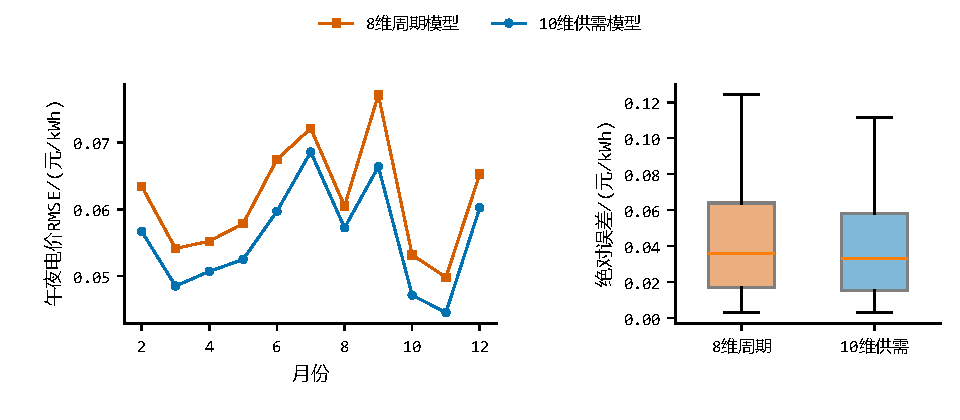
\includegraphics[width=\textwidth]{final_results/q4_price.pdf}
 \caption{两种午夜价格模型在相同48096槽上的预测误差。右图箱体为四分位区间，横线为中位数，须为5\%与95\%分位数，不表示置信区间。}
 \label{fig:q4-price}
\end{figure}
\begin{table}[H]
\centering\small
\caption{波动电价下两类完整方案的评价期结果}\label{tab:q4-annual}
\begin{tabular}{lrr}
\toprule
指标 & 方案4-2 & 方案4-3\\
\midrule
原计划费/元 & 13402862.29 & 12266424.93\\
上调费/元 & 0.00 & 1132763.34\\
下调退款/元 & 0.00 & -83052.64\\
紧急购电费/元 & 605747.24 & 223687.99\\
总费用/元 & 14008609.54 & 13539823.62\\
最终常规购电量/kWh & 20506017.8625 & 19865431.5040\\
紧急购电量/kWh & 112042.9064 & 46082.4095\\
非空方向反转/次 & 1757 & 6679\\
电芯等效满循环/次 & 463.6987 & 525.4197\\
\bottomrule
\end{tabular}
\end{table}


图\ref{fig:q4-monthly}给出各月总费用与紧急费占比，月总额保留各月天数差异；图\ref{fig:q4-daily-difference}进一步展示逐日费用差异，以正值表示方案4-3费用较低。不同季节的供需与价格共同影响结果，不能以月总费用直接替代日均效率指标。
\begin{figure}[H]
 \centering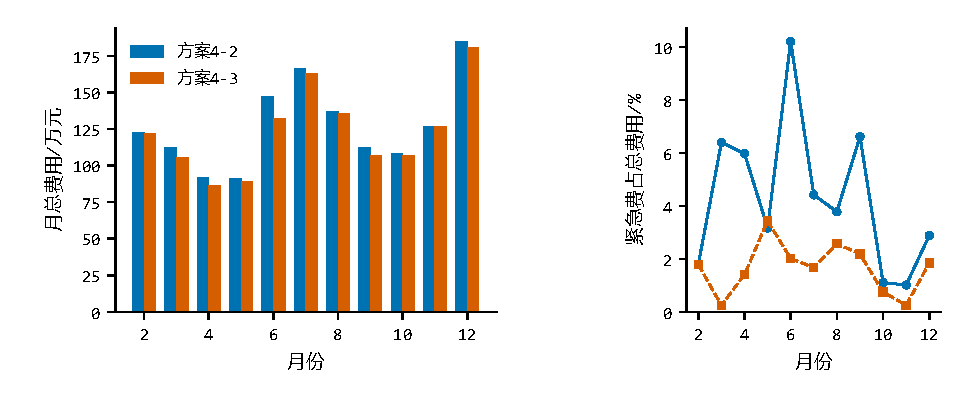
\includegraphics[width=\textwidth]{final_results/q4_monthly.pdf}
 \caption{两类完整方案的月度费用与紧急费占比。}
 \label{fig:q4-monthly}
\end{figure}
\begin{figure}[H]
 \centering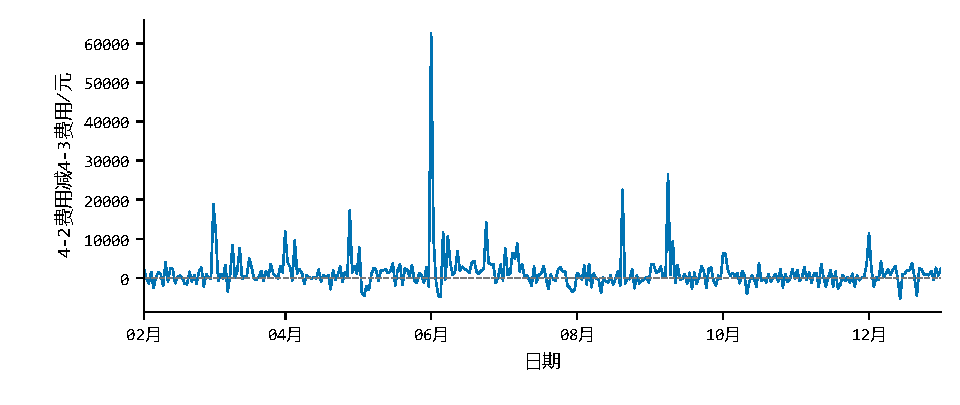
\includegraphics[width=\textwidth]{final_results/q4_daily_difference.pdf}
 \caption{评价期每日总费用差（方案4-2减方案4-3）。该差额反映两套完整策略的共同差异。}
 \label{fig:q4-daily-difference}
\end{figure}

\textbf{指定日期调度。}
方案4-2的指定槽与全天购电量见表\ref{tab:q4_4-2-final}，方案4-3的午夜计划与最终量见表\ref{tab:q4_4-3-original}、\ref{tab:q4_4-3-final}。两方案四个指定日的储能结果分别见表\ref{tab:q4_4-2-storage-47}、\ref{tab:q4_4-2-storage-140}、\ref{tab:q4_4-2-storage-234}、\ref{tab:q4_4-2-storage-323}和表\ref{tab:q4_4-3-storage-47}、\ref{tab:q4_4-3-storage-140}、\ref{tab:q4_4-3-storage-234}、\ref{tab:q4_4-3-storage-323}。紧急购电完整区间见表\ref{tab:q4_4-2-emergency}和表\ref{tab:q4_4-3-emergency}。
\begin{table}[H]
\centering\small
\caption{问题4-2指定日期的最终常规购电量（单位：kWh）}\label{tab:q4_4-2-final}
\begin{tabular}{lrrrr}
\toprule
时间段 & 3月20日 & 6月21日 & 9月23日 & 12月21日\\
\midrule
10:00--10:10 & 56.8021 & 0.0000 & 14.2668 & 0.0000\\
12:00--12:10 & 564.5003 & 0.0000 & 504.4275 & 999.2309\\
14:00--14:10 & 0.0000 & 0.0000 & 0.0000 & 0.0000\\
16:00--16:10 & 431.9505 & 252.1208 & 499.5770 & 1165.4219\\
18:00--18:10 & 675.7274 & 382.0389 & 718.5905 & 691.9762\\
20:00--20:10 & 121.2289 & 0.0000 & 97.0970 & 0.0000\\
全天电量 & 66523.2925 & 31152.4188 & 68627.2874 & 88185.5065\\
全天总费用/元 & 42360.91 & 16636.03 & 45477.18 & 68042.02\\
\bottomrule
\end{tabular}
\end{table}
\begin{table}[H]\centering\small
\caption{方案4-2四个指定日期的充放电量及起止储电量（kWh）}\label{tab:q4_4-2-storage-dates}
\begin{tabular}{lrrrr}\toprule
时间段或指标&3月20日&6月21日&9月23日&12月21日\\\midrule
\multicolumn{5}{l}{充电量（kWh）}\\
00:00--04:00&7396.6319&0.0000&8044.4697&4706.9660\\
04:00--08:00&1757.3799&0.0000&0.0000&0.0000\\
08:00--12:00&5819.2437&9757.9626&5059.8420&4424.1685\\
12:00--16:00&3399.7565&0.0000&2952.2254&7692.5936\\
16:00--20:00&0.0000&0.0000&0.0000&394.3369\\
20:00--24:00&1515.8655&0.0000&1810.3827&0.0000\\
\midrule
\multicolumn{5}{l}{放电量（kWh）}\\
00:00--04:00&87.3354&2467.5629&0.0000&193.1802\\
04:00--08:00&5318.2836&1870.8452&4995.7313&988.5520\\
08:00--12:00&2777.3772&0.0000&1893.2268&7041.4419\\
12:00--16:00&519.5389&0.0000&592.1208&3036.8150\\
16:00--20:00&6015.2029&4428.1966&6067.2634&5638.3036\\
20:00--24:00&2572.6178&3174.2822&2574.9749&3093.9648\\
\midrule
0:00储电量&1995.4658&6115.8675&3168.3459&6334.5799\\
24:00储电量&2638.0763&2786.2837&3122.9258&1595.3809\\
\bottomrule\end{tabular}\end{table}
\begin{table}[H]
\centering\small
\caption{方案4-2四个指定日期的紧急购电区间（kWh）}\label{tab:q4_4-2-emergency}
\setlength{\tabcolsep}{3pt}
\begin{tabular}{lrlrlrlr}
\toprule
\multicolumn{2}{c}{3月20日} & \multicolumn{2}{c}{6月21日} & \multicolumn{2}{c}{9月23日} & \multicolumn{2}{c}{12月21日}\\
时间段 & 电量 & 时间段 & 电量 & 时间段 & 电量 & 时间段 & 电量\\
\midrule
21:20--22:00 & 116.1019 & -- & -- & 15:00--15:10 & 7.7027 & 17:20--17:30 & 4.1823\\
合计 & 116.1019 & 合计 & 0.0000 & 合计 & 7.7027 & 合计 & 4.1823\\
\bottomrule
\end{tabular}
\end{table}

\begin{table}[H]
\centering\small
\caption{问题4-3指定日期的原计划购电量（单位：kWh）}\label{tab:q4_4-3-original}
\begin{tabular}{lrrrr}
\toprule
时间段 & 3月20日 & 6月21日 & 9月23日 & 12月21日\\
\midrule
10:00--10:10 & 0.0000 & 0.0000 & 0.0000 & 0.0000\\
12:00--12:10 & 447.5773 & 0.0000 & 294.9785 & 977.8658\\
14:00--14:10 & 0.0000 & 0.0000 & 0.0000 & 0.0000\\
16:00--16:10 & 642.1417 & 96.9398 & 524.6990 & 865.8055\\
18:00--18:10 & 632.4041 & 0.0000 & 723.2164 & 680.6723\\
20:00--20:10 & 114.6849 & 0.0000 & 0.3603 & 0.0000\\
全天电量 & 61441.5401 & 29640.7183 & 64616.1447 & 90372.9344\\
\bottomrule
\end{tabular}
\end{table}
\begin{table}[H]
\centering\small
\caption{问题4-3指定日期的最终常规购电量（单位：kWh）}\label{tab:q4_4-3-final}
\begin{tabular}{lrrrr}
\toprule
时间段 & 3月20日 & 6月21日 & 9月23日 & 12月21日\\
\midrule
10:00--10:10 & 0.0000 & 0.0000 & 0.0000 & 0.0000\\
12:00--12:10 & 500.6572 & 0.0000 & 294.9785 & 942.1100\\
14:00--14:10 & 0.0000 & 0.0000 & 0.0000 & 0.0000\\
16:00--16:10 & 642.1417 & 96.9398 & 524.6990 & 1412.1259\\
18:00--18:10 & 678.6308 & 0.0000 & 725.6931 & 705.7614\\
20:00--20:10 & 719.6935 & 0.0000 & 2.0019 & 0.0000\\
全天电量 & 63775.7995 & 30514.7960 & 65529.3019 & 92829.0596\\
全天总费用/元 & 42751.71 & 15553.81 & 43840.15 & 72598.29\\
\bottomrule
\end{tabular}
\end{table}
\begin{table}[H]\centering\small
\caption{方案4-3四个指定日期的充放电量及起止储电量（kWh）}\label{tab:q4_4-3-storage-dates}
\begin{tabular}{lrrrr}\toprule
时间段或指标&3月20日&6月21日&9月23日&12月21日\\\midrule
\multicolumn{5}{l}{充电量（kWh）}\\
00:00--04:00&7383.9974&901.4645&9446.8317&10107.0507\\
04:00--08:00&2543.5155&1613.5323&793.1483&1792.0683\\
08:00--12:00&2464.9699&9783.1738&4906.2508&4308.2839\\
12:00--16:00&6123.8121&0.0000&4744.6378&9238.4489\\
16:00--20:00&549.2050&25.8726&0.0000&228.1659\\
20:00--24:00&313.2254&2751.3906&1186.5006&1139.8274\\
\midrule
\multicolumn{5}{l}{放电量（kWh）}\\
00:00--04:00&310.9833&2485.0043&6.2947&150.7402\\
04:00--08:00&6656.0298&1485.0959&7126.9436&2520.6360\\
08:00--12:00&2677.3195&0.0000&1896.6157&7911.5199\\
12:00--16:00&254.7228&0.0000&443.0756&3404.2588\\
16:00--20:00&6628.0990&6420.2901&6359.8540&6181.9629\\
20:00--24:00&1410.7146&4539.5586&2706.0787&3708.6294\\
\midrule
0:00储电量&1947.9534&3317.7840&1731.7495&1210.4470\\
24:00储电量&1424.0526&1882.0483&2185.8209&1478.9384\\
\bottomrule\end{tabular}\end{table}
\begin{table}[H]
\centering\small
\caption{方案4-3四个指定日期的紧急购电区间（kWh）}\label{tab:q4_4-3-emergency}
\setlength{\tabcolsep}{3pt}
\begin{tabular}{lrlrlrlr}
\toprule
\multicolumn{2}{c}{3月20日} & \multicolumn{2}{c}{6月21日} & \multicolumn{2}{c}{9月23日} & \multicolumn{2}{c}{12月21日}\\
时间段 & 电量 & 时间段 & 电量 & 时间段 & 电量 & 时间段 & 电量\\
\midrule
09:30--10:00 & 100.0577 & 06:50--07:20 & 176.8897 & 20:10--20:20 & 10.2344 & 07:50--08:00 & 4.4020\\
-- & -- & -- & -- & -- & -- & 20:40--20:50 & 215.7174\\
合计 & 100.0577 & 合计 & 176.8897 & 合计 & 10.2344 & 合计 & 220.1194\\
\bottomrule
\end{tabular}
\end{table}


图\ref{fig:q4-dispatch}以9月23日展示电价、购电与储能轨迹。方案4-2受小时模式约束，方案4-3随日内预报修订剩余购电，两者产生不同的库存和功率变化。图中的电价预测均取午夜版本；方案4-3在后续发布时还会重新估计价格，并未始终保持午夜价格预测。
\begin{figure}[H]
 \centering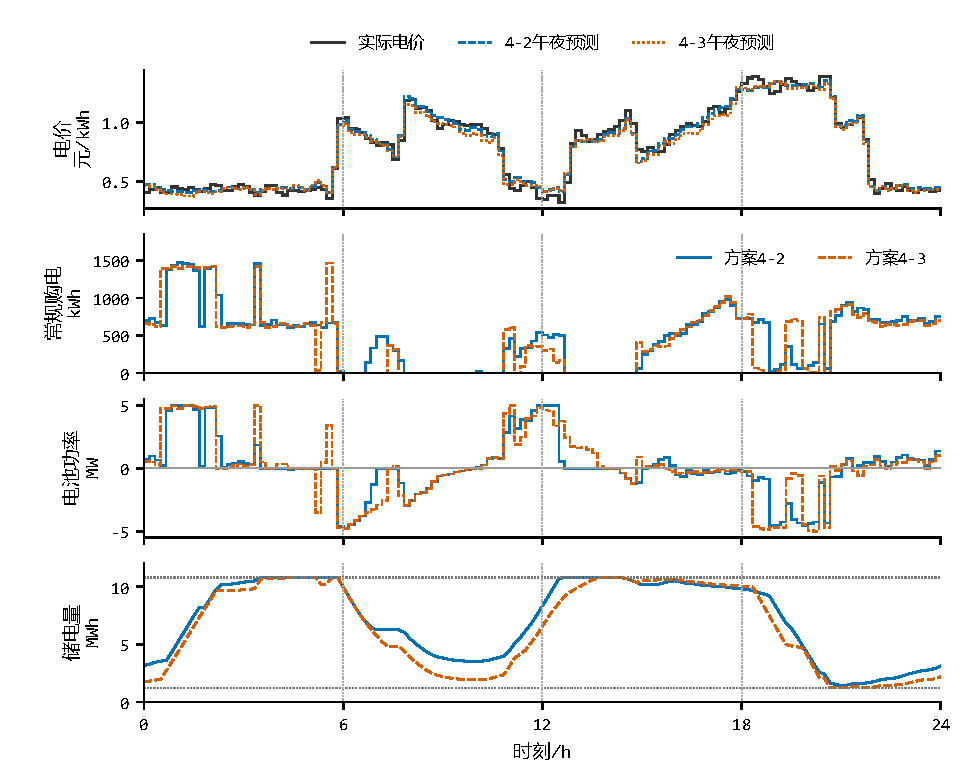
\includegraphics[width=\textwidth]{final_results/q4_dispatch.pdf}
 \caption{9月23日的电价、购电与储能运行轨迹。功率正值表示充电，负值表示放电；竖线为6、12、18时发布时刻，储电量水平虚线为安全边界。}
 \label{fig:q4-dispatch}
\end{figure}

\textbf{结果检验。}
逐槽能量平衡、SOC递推和跨日衔接通过核对，两方案实际同时充放电及紧急购电用于充电的槽数均为零，储电量与充放电功率满足题设边界。费用按式\eqref{eq:q4-cost}独立复算，完整购电策略分别保存于\texttt{result4-2.xlsx}、\texttt{result4-3.xlsx}。本节为按时间推进的开发年度回测，月度结果不构成独立跨年泛化检验。

\end{document}
